\section{Results}
\label{section:results}
%------------------------------------------------------------------------------------------
% Simulation

% Map
The SLAM map obtained during simulation is shown in Fig.\:\ref{fig:simulation_slam_map}.
\begin{figure}
    \centering
    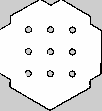
\includegraphics[width=\columnwidth]{images/simulation_SLAM_map.png}
    \caption{Map generated using SLAM in simulation.}
    \label{fig:simulation_slam_map}
\end{figure}
% Evaluation metrics
The performance of the simulated system in terms of the evaluation metrics has been summarized in Table.\:\ref{tab:simulation_metrics}.
\begin{table}
    \centering
    \resizebox{\columnwidth}{!}{\noindent\begin{tabular}{|c|c|} \hline
         \textbf{Number of collisions}  & \textbf{Processing time per sensor update (ms)}       \\ \hline
         $0$                            & Could not be measured                                 \\ \hline
    \end{tabular}}
    \caption{Evaluation metrics obtained during testing of the simulated system.}
    \label{tab:simulation_metrics}
\end{table}

%------------------------------------------------------------------------------------------
% Real world

% Map
The map obtained using SLAM during real-world deployment can be seen in Fig.\:\ref{fig:real_world_slam_map}.
\begin{figure}
    \centering
    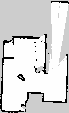
\includegraphics[width=\columnwidth]{images/real_world_SLAM_map.png}
    \caption{SLAM map obtained during real-world deployment of the developed system.}
    \label{fig:real_world_slam_map}
\end{figure}
% Evaluation metrics
The systems performance in real-world deployment is shown in Table\:\ref{tab:real_world_metrics}.
\begin{table}
    \centering
    \resizebox{\columnwidth}{!}{\noindent\begin{tabular}{|c|c|c|} \hline
         \textbf{Number of collisions}  & \textbf{Processing time per sensor update (ms)}       \\ \hline
         $0$                            & Could not be measured                                 \\ \hline
    \end{tabular}}
    \caption{Evaluation metrics obtained during real-world deployment and testing of the system.}
    \label{tab:real_world_metrics}
\end{table}


%------------------------------------------------------------------------------------------


%------------------------------------------------------------------------------------------
\begin{comment}
    
\end{comment}
%------------------------------------------------------------------------------------------